\subsection{Error Detection and Mitigation}
Dual Modular Redundancy (DMR) is the traditional approach for detecting faults,
where any difference between duplicated versions of components operating with the same state indicates 
an error.
Typically this is performed with two identical hardware units executing in lock step and
periodically comparing their outputs.

Redundancy is often not feasible in constrained systems like satellites
since it is inherently costly consuming area, power, time, or all of the above.
For this reason researchers have been interested in finding methods to
increase reliability with less redundancy but without increasing engineering effort.
The majority of research into this problem has primarily focussed on low level approaches,
with only a few investigations into how this can be achieved through HLS tools.

The majority of modern reliable HLS work has revolved around the idea of a component
library, where implementations of the same components with different resource to
reliability trade offs are selected during the allocation phase of the HLS tool
\cite{tosun2005reliability}, \cite{glass2007interactive}, \cite{hara2013cost}.
While these works do a great job at exploring the reliability trade offs they
all have the same assumption that reliability is equally important across
portions of the computation, but is this necessarily true?

A large number of studies within the software domain have explored the resilience of various applications
to the injection of soft errors, and found that there are clear regions of code that
are more critical than others LIST OF CITATIONS HERE.

In \cite{wong2006soft} the authors examined probabilistic
inference applications which are designed to be robust against noisy incomplete input
data to see if this also translated to resilience to soft errors.
Instruction level fault injection techniques were used to discover that such algorithms
have a natural ability to mask multiple data errors, however control flow errors were more
severe and tended to result in premature program termination.

Within the field of approximate computing there has also been interest in separating code into
critical and non-critical sections.
A notable example is EnerJ \cite{sampson2011enerj} where type
annotations indicate whether code regions should be precise or imprecise.
The type system then ensures the segregation of imprecise code from precise code allowing for the safe execution of imprecise code on approximate hardware.
Flikker \cite{liu2012flikker} has a similar approach where type-annotations are used to store data in
DRAM banks that are refreshed below the recommended manufacturers rate to save idle power consumption.  
For a selection of mobile application benchmarks they find that large portions of memory can be safely
stored in the low refresh DRAM with minimal impact on application results.

\begin{figure}[h]
\centering
%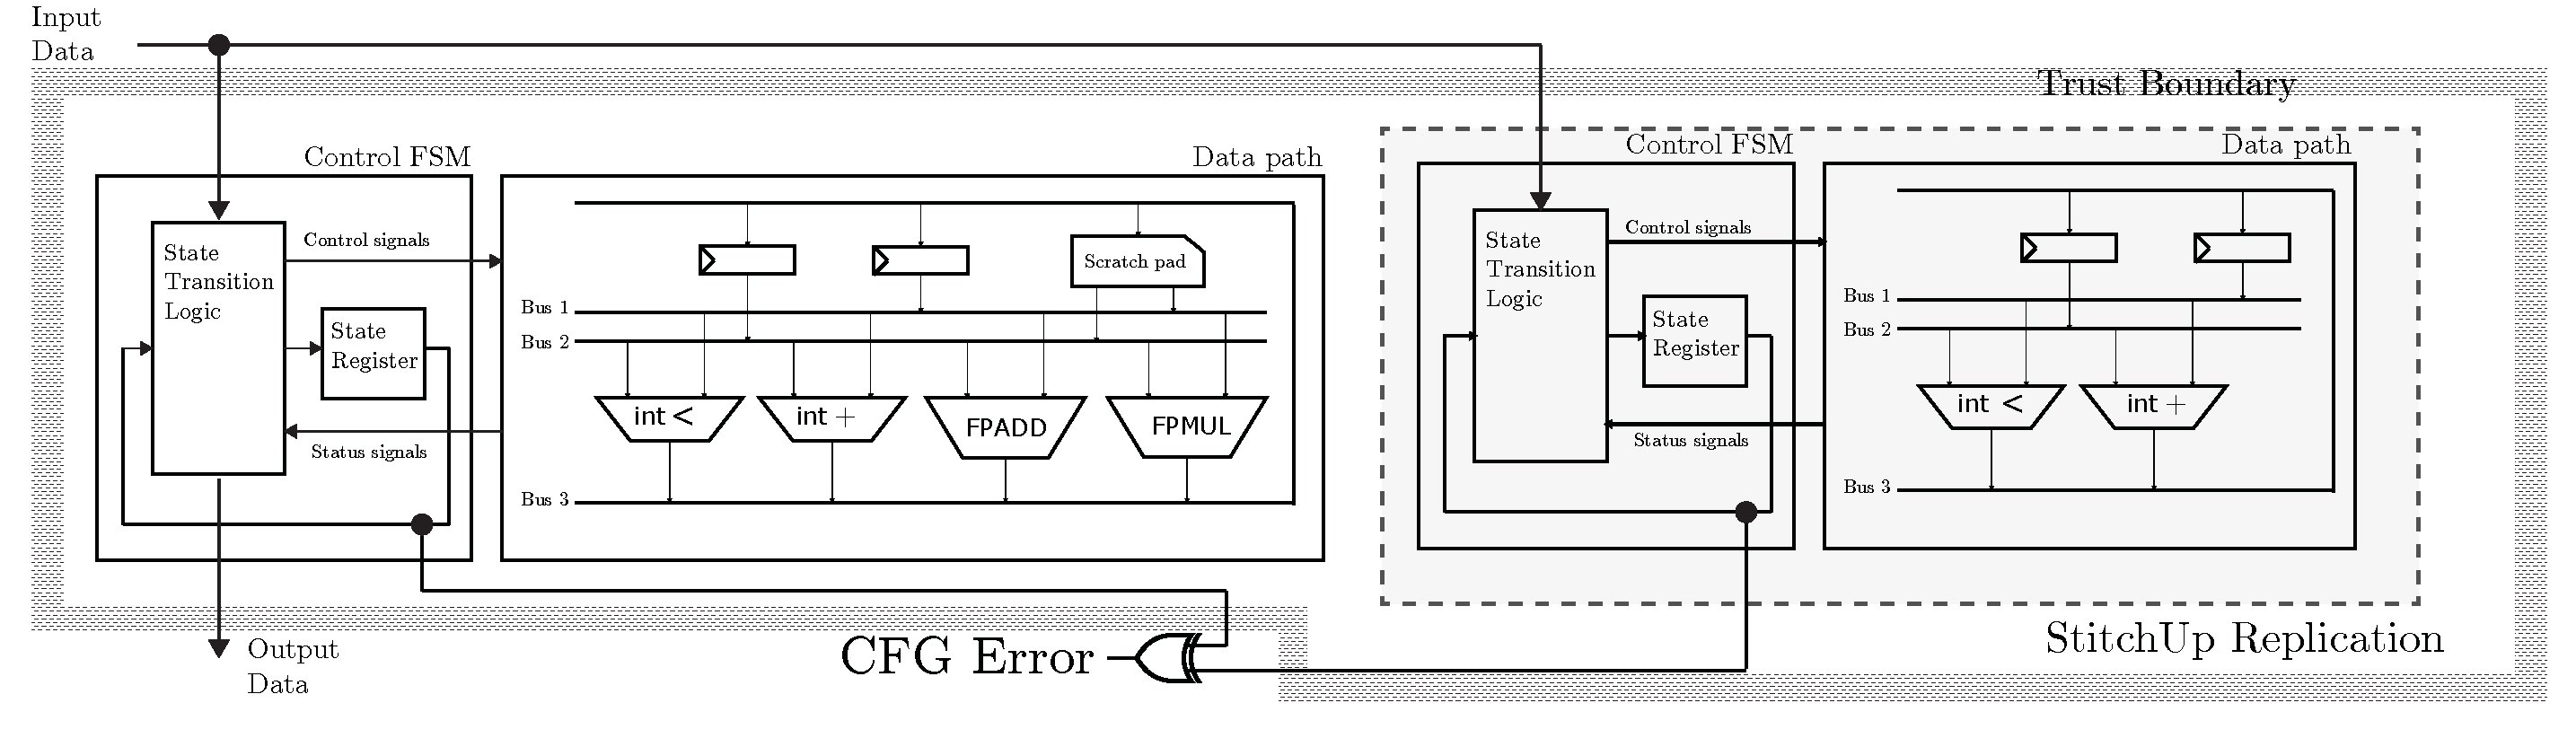
\includegraphics[width=7in]{./imgs/HLSArch.pdf}
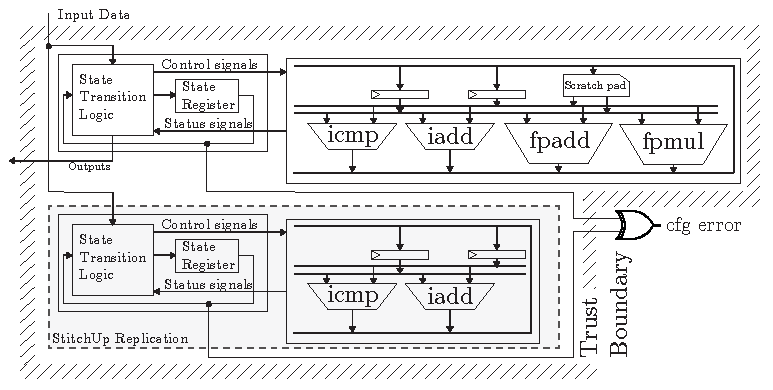
\includegraphics[width=3.5in]{./imgs/StitchUpReplication.pdf}
\caption{StitchUp Replication for the Matrix Multiplication example, with Trust Boundary}
\label{fig:HLSArch}
\end{figure}

\subsection{Fault Model}
A Soft Error or Single Event Upset is a random non-catastrophic error, where radiation causes
a perturbation to a circuit by temporarily altering a single signal or datum. 
Detecting and mitigating such errors is highly important in some fields, such as satellite design, 
where high design costs, harsh environments, and difficulties to repair once deployed make it necessary. 
However with the continuing increasing of semiconductor densities the current soft error mitigation
challenges experienced in space will be the future problems of terrestrial devices\cite{normand1996single}\cite{henkel2013reliable}.
%However these concerns are no longer restricted to niche fields
%since the shrinking of both device feature sizes and operating voltages make it increasingly likely 
%that ground level radiation sources can cause soft errors.
%This effect has been known about for some time \cite{normand1996single} and is related to 
%the reduction in critical charge required to cause an upset, this in turn broadens the spectrum of
%particles able to cause upsets such as muons with lower ionising power that are prevalent in terrestrial
%environments.
%Consequently, this concern is driving reliability as a first-class design constraint in the 
%development of digital systems.

In this work we shall focus on single \textbf{single} errors, assuming that only one SEU
can occur per clock cycle.
We shall also limit ourselves to SRAM based FPGA designs, although the protection scheme 
presented in this paper can be equally applied to VLSI designs.

In an FPGA design circuit descriptions are mapped into a collection of Logic Blocks, decribed in programmable look-up-tables,
which are routed together via programmable switchboxes.
Configuration data for both the look-up-tables and switchboxes are stored in a configuration memory, which means soft errors
can either change the functionality of Logic Blocks or can change the routing between them.
Block memory and flip-flops are also present in FPGA devices, where soft errors in these regions can alter the state of the circuit.
For this paper our \emph{fault model} assumes that a single soft error can occur at most every clock cycle, and that this error can effect block memory, configuration memory, and flip-flops. 
However our fault model does not include routing to and from our protected region to external I/O, such as DDR accesses.


